\documentclass[fleqn]{homework}

\student{Stephen Brennan (smb196)}
\course{EECS 477}
\assignment{Homework 5}
\duedate{November 23, 2015}

\usepackage{mathtools}
\usepackage{graphicx}
\usepackage{enumerate}

\begin{document}
  \maketitle

  \begin{problem}{1}
    \begin{question}
      Apply the capacity-scaling algorithm to the minimum cost flow problem in
      the figure.

      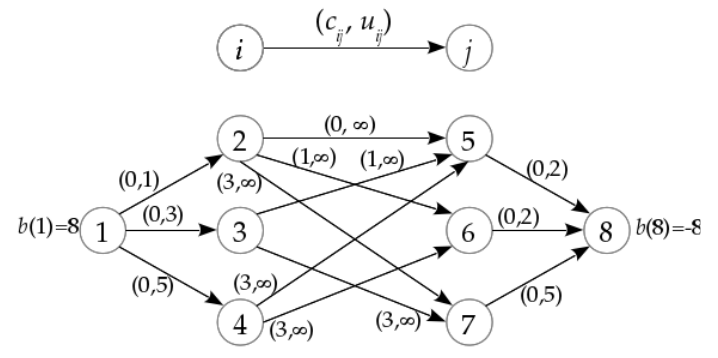
\includegraphics[width=0.6\textwidth]{p1.png}
    \end{question}
  \end{problem}

  \begin{problem}{2}
    \begin{question}
      In this problem, you will revisit the gambling chip game.  Assume that
      there are four chips of value 6, 5, 2, 7, and thus the game ends in two
      rounds.

      \begin{enumerate}[a.]
      \item Write the game in extensive form, and then convert the extensive
        form into strategic form.
      \item Model the strategic form game as a linear program and find the
        optimal mixed strategies for the two players.
      \item Assume that Bob uses his optimal mixed strategy.  Describe a
        deterministic strategy that Alice can use to maximize her winnings.
      \item Find an arrangement of at least two rounds for which the optimal
        strategy is deterministic for both players.
      \end{enumerate}
    \end{question}
  \end{problem}

  \begin{problem}{3}
    \begin{question}
      Consider a data structure implemented as a linked list containing $n$
      distinct items.  The data structure supports the operation
      \texttt{CONTAINS(item)}, which returns true if the list contains the given
      item and false otherwise.  A \texttt{CONTAINS(item)} takes time
      proportional to $O(p)$, where $p$ is the position of the item in the
      list.  Furthermore, once \texttt{CONTAINS(item)} has located the item, it
      can move it forward to any position between the first and the $p$th within
      the $O(p)$ time bound.  In this way, if the same item is being requested
      repeatedly, subsequent \texttt{CONTAINS(item)} will take less time.
      Consider an algorithm for determining whether to move the item forward and
      to which location.

      \begin{enumerate}[a.]
      \item Show that $p \ge n$ in the worst-case for any deterministic
        algorithm.
      \item Use Yao's principle to show that $p \ge (n+1) / 2$ in the worst case
        for any randomized algorithm.
      \end{enumerate}
    \end{question}

    This situation can be represented as a two person zero-sum game, where the
    payoff is the the runtime of the algorithm.  The two players are $A$, the
    algorithm, and $I$, the input.  $A$ tries to minimize the runtime, and $I$
    tries to maximize it.

    \begin{enumerate}[a.]
    \item A deterministic algorithm means that $A$ is using a pure strategy
      (such as ``always move the element to the front'' or ``always move the
      element to $\lfloor p/2 \rfloor$'', etc).  In this case, there is always a
      deterministic strategy that calls \texttt{CONTAINS} on the last item in
      the list each time.  This makes the worst-case payoff $n$ for any
      deterministic strategy of $A$.
    \item For the purpose of this question, we will define the game as a series
      of $n$ rounds ($n$ calls and $n$ executions of the algorithm).  In order
      to determine what the worst-case $p$ would be if $A$ used a randomized
      strategy, we look at the worst-case payoff for this game.  If we think of
      $x$ and $i$ as mixed and pure strategies for $I$ (maximizing player), and
      $y$ and $j$ as mixed and pure strategies for $A$ (minimizing player), then
      the worst-case payoff for the algorithm is:

      \begin{equation*}
        \min_y \max_i H(i,y)
      \end{equation*}

      According to Yao's principle, this follows the inequality:

      \begin{equation*}
        \min_y \max_i H(i,y) \ge \min_j H(x,j) \forall x
      \end{equation*}

      Consider the following mixed strategy $x$: select any ordering of items 1
      through $n$, and call \texttt{CONTAINS} on each one in order.  In this
      case, the optimal strategy $j$ is not to move any element forward in the
      list, because the input will never call \texttt{CONTAINS} on that element
      again.  The payoff of this strategy is:

      \begin{equation*}
        \min_j H(x, j) = \sum_{k=1}^n k = \frac{n(n+1)}{2}
      \end{equation*}

      Since this is over a ``game'' of $n$ calls, the worst-case runtime $p$ for
      a single call to the algorithm is $p \ge \frac{n+1}{2}$.
    \end{enumerate}
  \end{problem}

\end{document}